% Auto-generated by generate_report.py — do not edit manually
% Preamble mirrors oxengthesis.cls so figures match the body text:
% Carlito as main font, Latin Modern Math via unicode-math.
\documentclass[border=6pt]{standalone}
\usepackage{fontspec}
\setmainfont{Carlito}
\usepackage{unicode-math}
\setmathfont{Latin Modern Math}
\usepackage{pgfplots}
\pgfplotsset{compat=1.18}
\usepgfplotslibrary{groupplots}
\usetikzlibrary{patterns,positioning}
\begin{document}
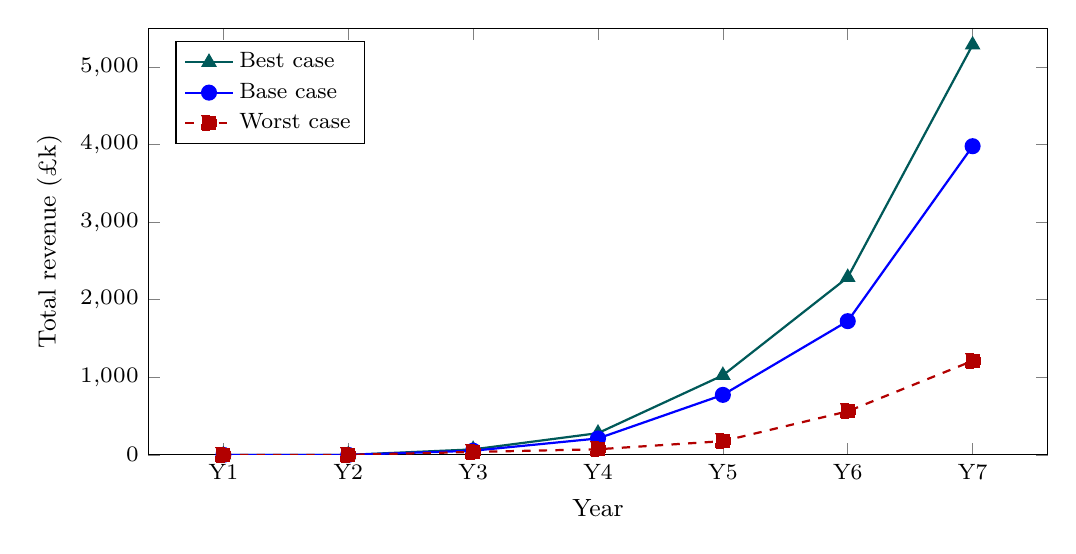
\begin{tikzpicture}
    \begin{axis}[
            width=13cm,
            height=7cm,
            xlabel={Year},
            symbolic x coords={Y1,Y2,Y3,Y4,Y5,Y6,Y7},
            xtick=data,
            legend style={
                font=\footnotesize,
                at={(0.02,0.98)},
                anchor=north west,
                legend cell align={left},
            },
            tick label style={font=\footnotesize},
            label style={font=\small},
        ylabel={Total revenue (\pounds k)},
        ymin=0, ymax=5500,
        legend pos=north west,
    ]
    \addplot[thick,teal!70!black,mark=triangle*,mark size=2.5pt] coordinates {(Y1,0.0) (Y2,0.0) (Y3,70.6) (Y4,280.1) (Y5,1025.1) (Y6,2288.1) (Y7,5284.9)};
    \addplot[thick,blue,mark=*,mark size=2.5pt] coordinates {(Y1,0.0) (Y2,0.0) (Y3,53.5) (Y4,211.7) (Y5,773.4) (Y6,1723.8) (Y7,3979.0)};
    \addplot[thick,red!70!black,mark=square*,mark size=2.5pt,dashed] coordinates {(Y1,0.0) (Y2,0.0) (Y3,37.4) (Y4,72.4) (Y5,177.0) (Y6,561.2) (Y7,1211.8)};
    \legend{Best case, Base case, Worst case}
    \end{axis}
\end{tikzpicture}

\end{document}
